\newpage
\vspace{3mm}

\subsubsection{Μελέτη των N-bit Predictors για σταθερό Hardware overhead}
Στο σημείο αυτό επαναλαμβάνεται η μελέτη της απόδοσης των N-bit Predictors για
διαφορετικές τιμές του N = 1, 2, 2b, 4, με τη διαφορά ότι θα μελετήσουμε την
επίδοση σε συνδυασμούς που αντιστοιχούν σε σταθερό hardware overhead 32Κ. \\

\noindent Ακολουθούν τα διαγράμματα που προέκυψαν και ο σχετικός σχολιασμός
τους:
\vspace{1em}

   \begin{minipage}{\textwidth}
      \begin{center}
         \fbox{\textlatin{\textbf{\textit{403-gcc}}}}\\
         \vspace{3mm}
         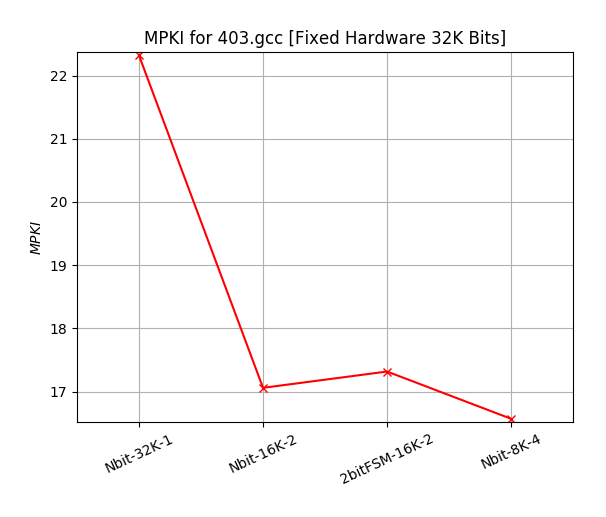
\includegraphics[width=0.65\textwidth, frame]{./graphs/4-2ii/403-gcc.png}
         \vspace{6mm}
      \end{center}
   \end{minipage}

   \begin{minipage}{\textwidth}
      \begin{center}
         \fbox{\textlatin{\textbf{\textit{429-mcf}}}}\\
         \vspace{3mm}
         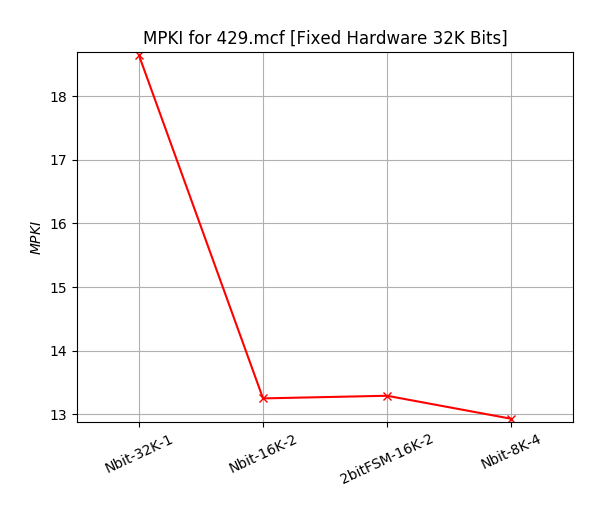
\includegraphics[width=0.65\textwidth, frame]{./graphs/4-2ii/429-mcf.png}
         \vspace{6mm}
      \end{center}
   \end{minipage}

   \begin{minipage}{\textwidth}
      \begin{center}
         \fbox{\textlatin{\textbf{\textit{434-zeusmp}}}}\\
         \vspace{3mm}
         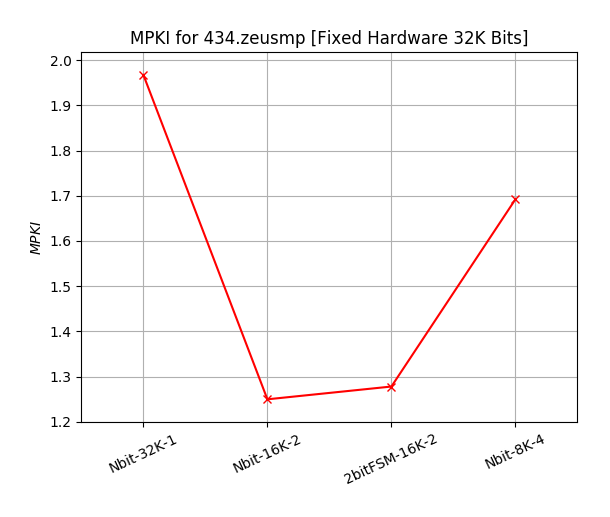
\includegraphics[width=0.65\textwidth, frame]{./graphs/4-2ii/434-zeusmp.png}
         \vspace{6mm}
      \end{center}
   \end{minipage}

   \begin{minipage}{\textwidth}
      \begin{center}
         \fbox{\textlatin{\textbf{\textit{436-cactusADM}}}}\\
         \vspace{3mm}
         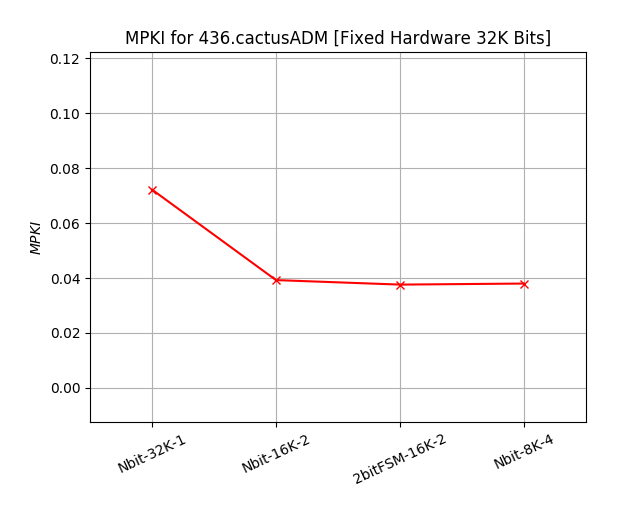
\includegraphics[width=0.65\textwidth, frame]{./graphs/4-2ii/436-cactusADM.png}
         \vspace{6mm}
      \end{center}
   \end{minipage}

   \begin{minipage}{\textwidth}
      \begin{center}
         \fbox{\textlatin{\textbf{\textit{445-gobmk}}}}\\
         \vspace{3mm}
         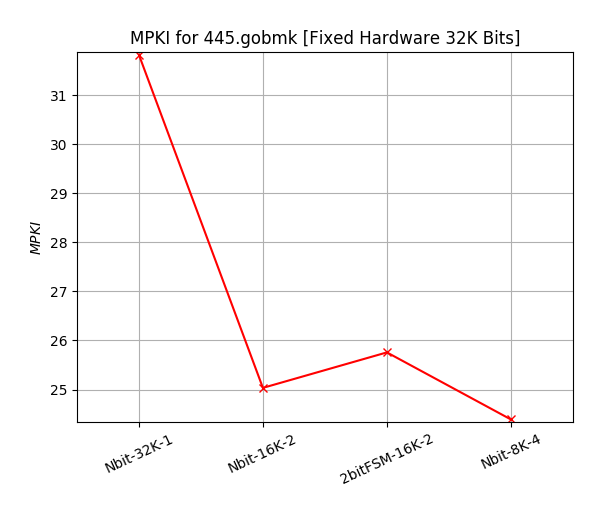
\includegraphics[width=0.65\textwidth, frame]{./graphs/4-2ii/445-gobmk.png}
         \vspace{6mm}
      \end{center}
   \end{minipage}

   \begin{minipage}{\textwidth}
      \begin{center}
         \fbox{\textlatin{\textbf{\textit{450-soplex}}}}\\
         \vspace{3mm}
         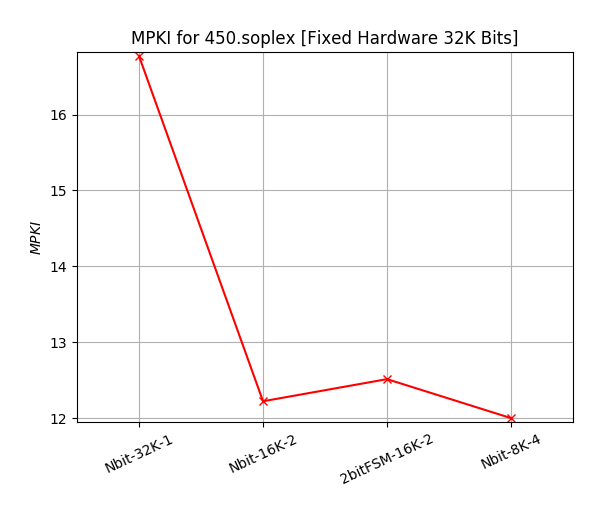
\includegraphics[width=0.65\textwidth, frame]{./graphs/4-2ii/450-soplex.png}
         \vspace{6mm}
      \end{center}
   \end{minipage}

   \begin{minipage}{\textwidth}
      \begin{center}
         \fbox{\textlatin{\textbf{\textit{456-hmmer}}}}\\
         \vspace{3mm}
         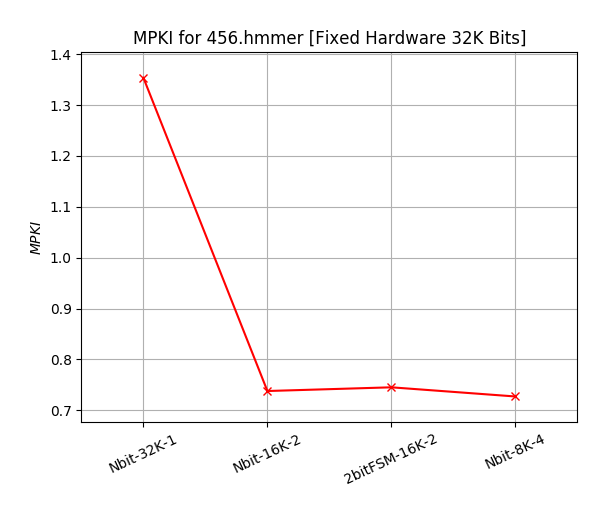
\includegraphics[width=0.65\textwidth, frame]{./graphs/4-2ii/456-hmmer.png}
         \vspace{6mm}
      \end{center}
   \end{minipage}

   \begin{minipage}{\textwidth}
      \begin{center}
         \fbox{\textlatin{\textbf{\textit{458-sjeng}}}}\\
         \vspace{3mm}
         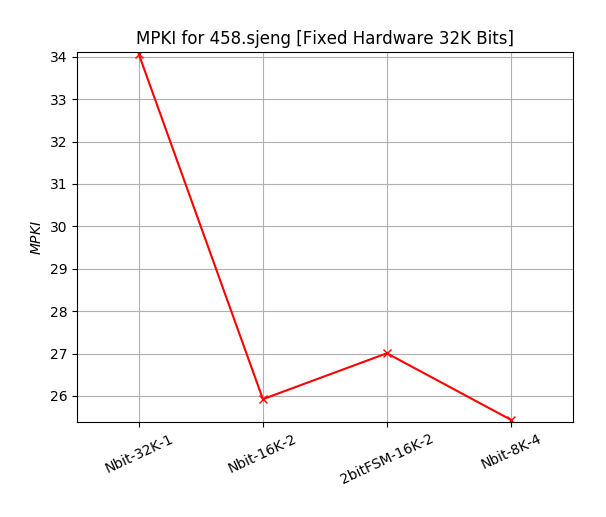
\includegraphics[width=0.65\textwidth, frame]{./graphs/4-2ii/458-sjeng.png}
         \vspace{6mm}
      \end{center}
   \end{minipage}

   \begin{minipage}{\textwidth}
      \begin{center}
         \fbox{\textlatin{\textbf{\textit{459-GemsFDTD}}}}\\
         \vspace{3mm}
         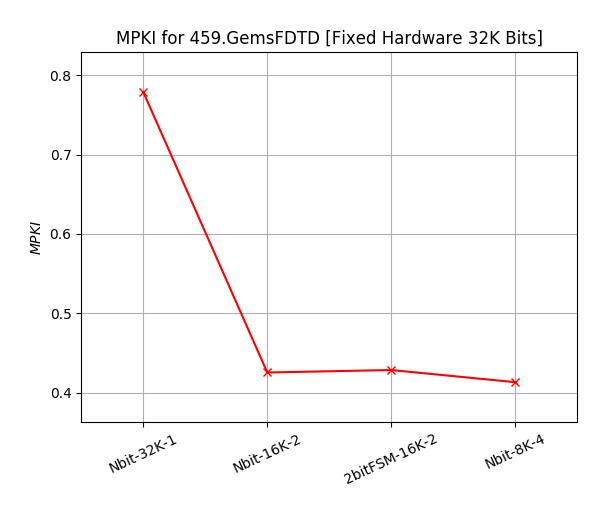
\includegraphics[width=0.65\textwidth, frame]{./graphs/4-2ii/459-GemsFDTD.png}
         \vspace{6mm}
      \end{center}
   \end{minipage}

   \begin{minipage}{\textwidth}
      \begin{center}
         \fbox{\textlatin{\textbf{\textit{471-omnetpp}}}}\\
         \vspace{3mm}
         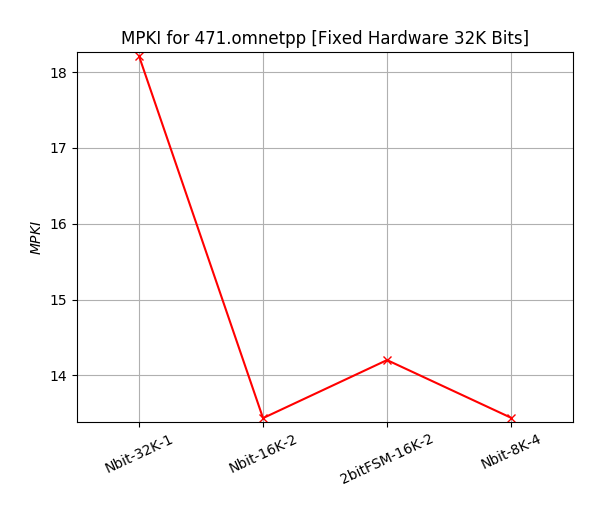
\includegraphics[width=0.65\textwidth, frame]{./graphs/4-2ii/471-omnetpp.png}
         \vspace{6mm}
      \end{center}
   \end{minipage}

   \begin{minipage}{\textwidth}
      \begin{center}
         \fbox{\textlatin{\textbf{\textit{473-astar}}}}\\
         \vspace{3mm}
         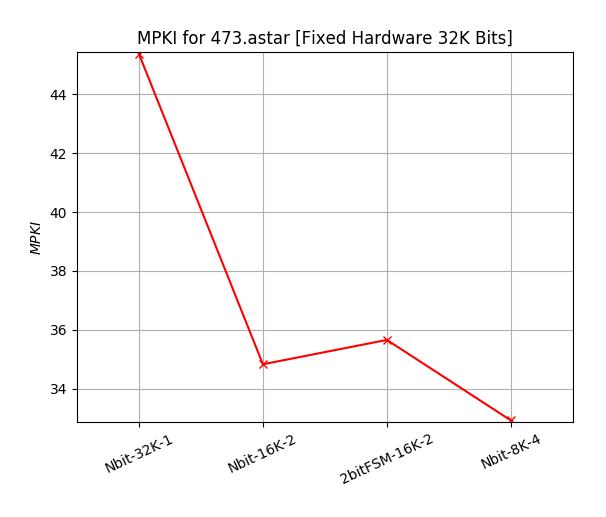
\includegraphics[width=0.65\textwidth, frame]{./graphs/4-2ii/473-astar.png}
         \vspace{6mm}
      \end{center}
   \end{minipage}

   \begin{minipage}{\textwidth}
      \begin{center}
         \fbox{\textlatin{\textbf{\textit{483-xalancbmk}}}}\\
         \vspace{3mm}
         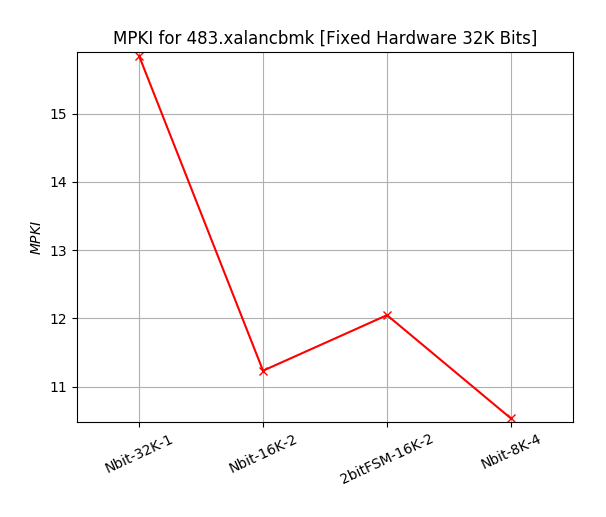
\includegraphics[width=0.65\textwidth, frame]{./graphs/4-2ii/483-xalancbmk.png}
         \vspace{6mm}
      \end{center}
   \end{minipage}

   \begin{minipage}{\textwidth}
      \begin{center}
         \fbox{\textlatin{\textbf{\textit{Geometric Average}}}}\\
         \vspace{3mm}
         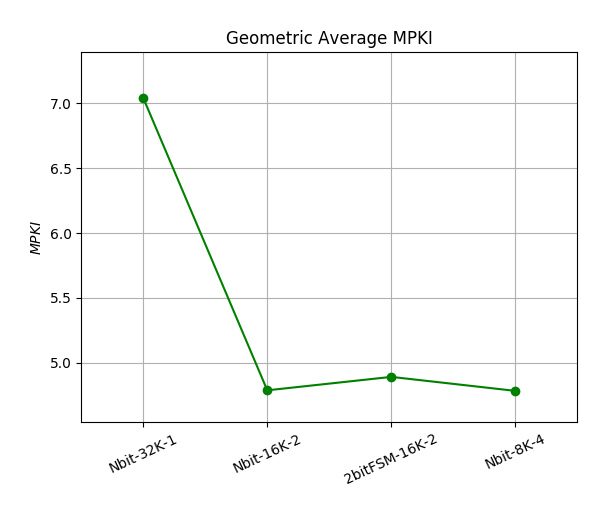
\includegraphics[width=0.65\textwidth, frame]{./graphs/4-2ii/mean.png}
         \vspace{6mm}
      \end{center}
   \end{minipage}

\paragraph{Συμπεράσματα-Σχόλια}
   Παρατηρούμε πως και στους νέους συνδυασμούς για σταθερό υλικό, η καμπύλες 
   μοιάζονυ με του προγηγούμενου ερωτήματος και τα συμπεράσματα είναι ανάλογα.

    Από της μορφές των καμπυλών στα παραπάνω διαγράμματα παρατηρούμε πως 11 στα
    12 benchmarks παρουσιάζουν βελτίωση καθώς το πλήθος των bits του predictor
    αυξάνει, δηλάδή η μετρική dMPKI φθίνει καθώς τα bits αυξάνονται, παρά την
    μείωση του πλήθος των predictors. Η μόνη διαφορετική ως προς την μορφή
    καμπύλη αντιστοιχεί στο μετρόπρόγραμμα 434.zeusmp για το οποίο το μικρότερο
    MPKI αντιστοιχεί σε 2-bit predictor.

   Λαμβάνοντας υπ'όψιν το διάγραμμα των γεωμετρικών μέσων, αλλά και την επίδοση
   με βάση τα επιμέρους διαγράμματα, μπορούμε να αποφανθούμε πως
   \textbf{καλύτερη επιλογή είναι ο 4-bit Predictor με 8Κ entries}. Εναλλακτικά
   θα μπορούσε να επιλαγεί και ο 2-bit Predicotr με 16Κ entries, αφού αποδίδει
   επίσης σχετικά καλά.

